\documentclass{article}

\usepackage[left=1in,right=1in,top=1in,bottom=1in]{geometry}
\usepackage{graphicx}
\usepackage{setspace}
\usepackage{float}
\usepackage{caption}
\usepackage{chngpage}
\usepackage{achemso}
\setkeys{acs}{usetitle=true}
\usepackage[affil-it]{authblk}

% put in paragraph spacing
\setlength{\parskip}{0.2cm}

\title{\textbf{Utilizing Machine Learning to Accelerate Automated Assignment of Backbone NMR Data}}

\author{Joel Venzke, David Mascharka, Paxten Johnson, Rachel Davis, Katie Roth, Leah Robison, Adina Kilpatrick and Timothy Urness*}
\affil{Department of Mathematics and Computer Science and the Department of Physics and Astromony,\\Drake University, Des Moines, Iowa\\\vspace{0.5cm}*Joel Venzke: joel.venzke@drake.edu\\Timothy Urness: timothy.urness@drake.edu}

\begin{document}

\maketitle

\begin{abstract}
Nuclear magnetic resonance (NMR) spectroscopy is a powerful method for determining three-dimensional structures of biomolecules, including proteins. In a critical step of the structure determination process for proteins, measured NMR values are assigned to specific amino acids in the protein primary sequence. Unfortunately, current manual techniques for the assignment of NMR data are time-consuming and susceptible to error. Many algorithms have been developed to automate the process, with various strengths and weaknesses. The algorithm described in this paper works to overcome the obstacles others have met by utilizing machine learning to predict amino acid type, thereby increasing assignment speed. The program also generates place-holders to accommodate missing data and recurring amino acids with unique chemical characteristics, namely proline. This approach is able to speed up the process of assignment by almost three orders of magnitude while maintaining high accuracy when compared to a previously assigned set.
\end{abstract}

\noindent\textbf{KEYWORDS}\\
Protein Sequencing, Machine Learning, NMR, Artificial Intelligence, Proteins, Bioinformatics

\noindent \textbf{INTRODUCTION}\\
NMR spectroscopy is a powerful method for obtaining atomic-resolution three-dimensional protein structures, as well as assessing changes in protein conformations or motions due to mutations or interactions with ligands or other biomolecules. Determining a protein's structure is essential for understanding its function and alterations in function, which often lead to disease. The analysis of Nuclear Magnetic Resonance (NMR) data, in particular the sequence-specific assignment of backbone and side-chain protein resonances, is an error-prone and time-consuming step during protein structure determination by NMR spectroscopy \cite{aria}. This paper describes a computational algorithm that utilizes machine learning in the process of automating the assignment of backbone protein NMR resonances.
\\\\
\noindent \textbf{BACKGROUND}\\
NMR spectroscopy experiments generate information on several variables that can be used in the determination of protein structures. In particular, essential information is provided by the chemical shifts of NMR-active nuclei present in proteins, including hydrogen and isotopes of carbon and nitrogen. The chemical shift is a quantifier for the deviation in the resonant frequency of a nucleus from its value in a structure-free environment, and therefore provides information on the local conformation. Measuring the chemical shifts of all or most of the nuclei in a protein is the first step in determining its structure by NMR spectroscopy. An important set of protein chemical shifts are those corresponding to the nuclei in the backbone of the protein polypeptide chain, including the amide nitrogen (N), attached hydrogen (H), and the alpha and beta carbons ($C_{\alpha}$ and $C_{\beta}$) of each residue. Chemical shift values are measured using various three-dimensional NMR experiments, and then matched to the individual residues in the protein in a process called sequential assignment.	
			
Triple resonance experiments on hydrogen, nitrogen and carbon nuclei are the method of choice for proteins and other large biomolecules, because they can greatly decrease the amount of spectral overlap in data. Typical experiments for the assignment of backbone resonances include HNCA, HN(CO)CA, HNCACB, and CBCA(CO)NH or HN(CO)CACB2. These experiments transfer magnetization over the protein polypeptide chain, and thus connect different spin systems through covalent bonds. A spin system essentially contains all resonances belonging to a particular residue in the protein sequence. The order of elements in experiment names indicates the order in which magnetization is passed down the line of nuclei, resonances in parentheses being used only for transfer to the next nucleus. All these experiments produce NMR spectra with common H-N resonance correlations, and provide connectivities between neighboring residues. For example, the HNCACB experiment identifies the chemical shifts corresponding to the $C_{\alpha}$ and $C_{\beta}$ nuclei of each residue in the protein chain (residue i), as well as the immediately preceding residue (residue $i-1$). In this experiment, resonances corresponding to residue $i$ can usually be distinguished from the $i-1$ values due to their higher intensity. However, ambiguities can arise if the intensities are comparable or if chemical shift values overlap. These ambiguities can be resolved by using additional experiments. For example, the CBCA(CO)NH experiment yields the chemical shifts of the preceding residue only, unambiguously identifying $i$ and $i-1$ values. Using all inter-residue connectivities, a chain of correlations through the protein backbone chemical shifts can be established. The pattern of sequentially-linked chemical shift values reflects the linear arrangement of individual residues in the protein sequence. This pattern is then matched to the protein sequence through certain residues with characteristic $C_{\alpha}$ and $C_{\beta}$ chemical shift values that uniquely identify them. Thus, each measured chemical shift is assigned to a protein residue and can then be used to infer structural information about the biomolecule.
\\\\
\noindent \textbf{SEQUENTIAL ASSIGNMENT STRATEGIES}
\begin{figure}[b]
	\caption{A sequence can be placed in order by matching $C_{\alpha}$ and $C_{\beta}$ values}
	\label{fig:joel_figure}
	\begin{center}
		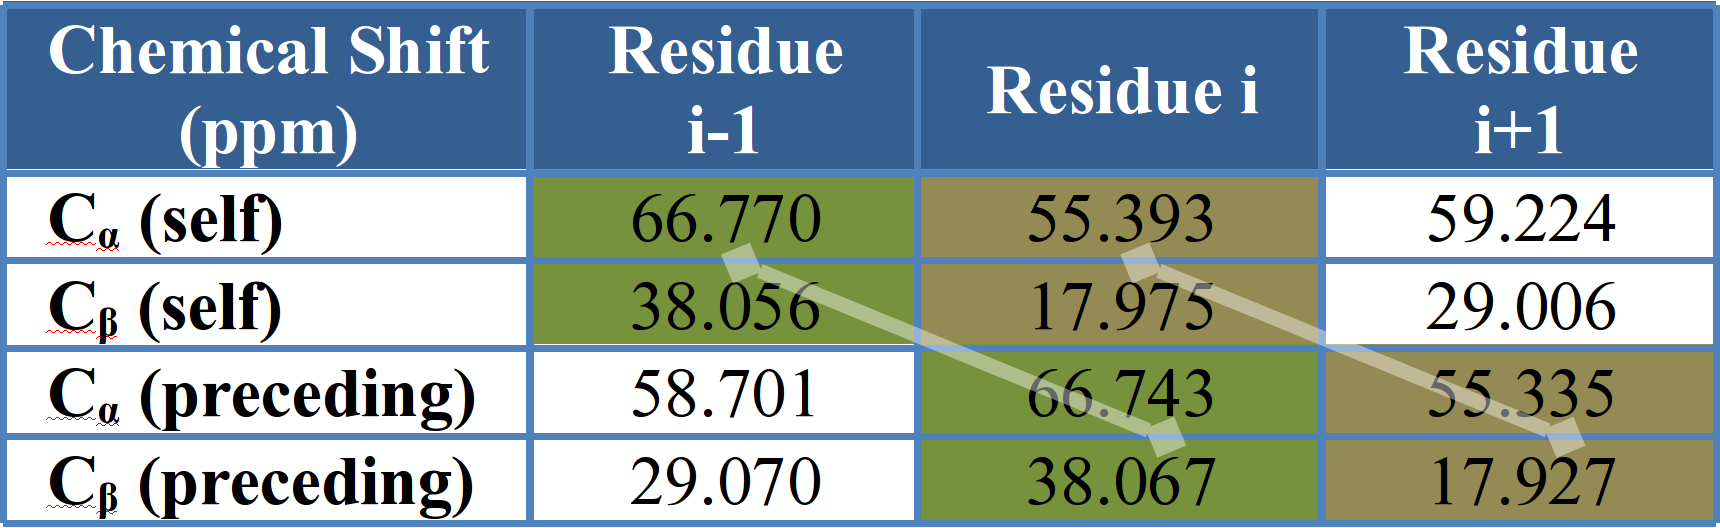
\includegraphics[keepaspectratio=true, width=0.7\textwidth]{residue_thingy}
	\end{center}
\end{figure}

The sequential assignment of backbone chemical shifts can be done manually or in an automated fashion. Both approaches follow similar strategies. The process starts by identifying the chemical shifts of $i$ and $i-1$ residues from a set of three-dimensional NMR experiments. In the early days of NMR spectroscopy, these chemical shifts were measured using a ruler \cite{guntert}. Nowadays, many computer programs, such as NMRPipe \cite{nmrpipe} and SPARKY \cite{goddard}, can be used to process, analyze and visualize NMR data. After grouping chemical shifts into spin systems, sequential spin systems are linked into increasingly larger segments by matching $i-1$ and $i$ values. This process can be seen in Figure~\ref{fig:joel_figure}. In parallel, the spin systems are classified into possible residue types, using a set of established chemical shift values for each of the 20 common amino acids found in proteins. For example, alanines have $C_{\alpha}$ and $C_{\beta}$ chemical shifts ranging from approximately 50 to 56 ppm (parts-per-million), and 17 to 25 ppm, respectively; glycines have unique $C_{\alpha}$ values in the 45 ppm region, and threonines have distinctive $C_{\beta}$ values in the 68-73 ppm range\cite{wishart, wang}. Using the residue type information, the linked segments from the resonance sequential walk are iteratively mapped onto the protein primary sequence. 

When performed manually, the assignment process is time-consuming and prone to errors. If chemical shifts values overlap, multiple matches between $i$ and $i-1$ values are possible. The classification of spin systems into amino acid types also has a high potential for error, as the spin systems can look identical or very similar even for very different amino acids. In recent years, advances in computer technology, accompanied by the increased use of NMR spectroscopy in drug design and structural genomics initiatives, have created a push for the automation of various steps in the NMR structure determination process \cite{moseley}. These automated methods decrease the time needed to complete the assignment, and attempt to minimize the risk of human error and subjectivity. A wide variety of algorithms and software packages for the assignment of backbone chemical shifts exist \cite{guntert}, including GARANT \cite{garant}, AutoAssign \cite{moseley,zimmerman} and MARS \cite{mars}.

Our algorithm utilizes elements from these existing programs, such as cost analysis, sorting amino acids into groups. Our algorithm employs novel concepts from machine learning to accelerate the assignment process.
\\\\
\noindent\textbf{MACHINE LEARNING}\\
Machine learning provides algorithms that learn from attributes in the input data to increase performance. Supervised learning, a field of machine learning, builds a model based on numerous data elements and their respective labels. The result is a mathematical model that predicts a label given a set of input attributes. By discovering patterns and trends in the data, machine learning algorithms provide excellent solutions for building models to generalize from large amounts of collected data with potentially many attributes, a task that is often difficult or impossible by other means.

Machine learning offers a natural solution to the problem of determining amino acid type from NMR chemical shift values. The overlap between the normal range of $C_{\alpha}$ and $C_{\beta}$ values between many amino acids makes it difficult to infer the type of residue based solely on chemical shift information. Machine learning algorithms offer a unique approach to this problem and achieve excellent accuracy.

There are several supervised machine learning algorithms that can be applied to improve automated assignment strategies. The J4.8 algorithm \cite{j48_algorithm} builds a decision tree model. This means that the data is split based on a comparison to an attribute of the data, with a branch for each possible outcome of the test. At the end of the tree, the leaf, is the predicted label. In our case this is the amino acid type. To classify a new value, a datapoint begins at the root of the tree and moves through until a leaf is encountered. The encountered leaf is the predicted value for that datapoint. To construct the tree, the attribute test used at each branch is the one that partitions the set in the most useful manner.

The Logistic Model Tree, or LMT \cite{lmt_algorithm}, is another tree-based algorithm. In contrast to the J4.8 algorithm, LMT constructs a tree with logistic regression functions at each branch rather than an attribute test. Logistic regression attempts to model class probabilities with linear functions (Hall). The weights used for each function can be learned to split each class in a way somewhat analogous to the split in J4.8 described above.

The Decision Table algorithm \cite{decisiontable_algorithm} is comprised of a set of features and a set of labeled data. To classify a new datapoint, the set of labeled data is searched for a match with the new point, considering only the features in the feature set. If no matches are found, the majority class of the labeled data is used. Otherwise, the majority class of the matches is used.
\\\\
\noindent\textbf{PROGRAM DEVELOPMENT}\\
Our goal is to create an automated program for the assignment of protein backbone chemical shifts that can deliver quality results in a small amount of time without the use of a supercomputer. Our program implements group sorting, machine learning, filtered amino acid selection, and careful cost calculations. The algorithm completes resonance assignment in six steps: (1) the NMR chemical shifts and the protein sequence are used to fill data structures; (2) the protein sequence is processed and empty data structures are initialized for missing data; (3) the machine learning model assigns possible amino acid types to each spin system; (4) filtering is applied to locate chemical shift values that could potentially be assigned to residue 1 in the protein sequence; (5) the search continues with the best assignments until all chemical shift data is assigned; (6) the best solution is recorded and the process is terminated. 

Before the algorithm begins the assignment process, machine learning is used to build a model for predicting amino acid type. After the model is trained, the pre-processing component of the algorithm (steps 1 to 3) begins. Pre-processing is where our research has made significant advances: by predicting amino acid types with machine learning algorithms, the assignment time is decreased significantly. Machine learning allows the data to be filtered, significantly reducing the branching factor. The algorithm is then able to intelligently search the remaining possibilities for the best assignment (steps 4 to 6). 
\\\\
\noindent\textbf{METHODS}\\
\noindent\textit{MACHINE LEARNING DATA COLLECTION}\\
The training dataset for the machine learning algorithm was obtained from the Biological Magnetic Resonance Bank (BMRB), a database of NMR chemical shifts hosted by the University of Wisconsin at Madison \cite{biomagresbank}. We initially identified 9,736 datasets containing chemical shifts for the $C_{\alpha}$ and $C_{\beta}$ resonances of 689,977 residues. In order to improve both accuracy and generalization, and to prevent the algorithm from fitting extraneous data, it was necessary to remove outliers from the published datasets. By inspecting statistics available on the BMRB site, we excluded chemical shift values outside three standard deviations of the mean for each amino acid type. This gave us 681,363 pairs of $C_{\alpha}$ and $C_{\beta}$ values to use for training.
\\\\
\noindent\textit{PRE-PROCESSING}\\
Step 1 of our algorithm consists of reading the chemical shift values and the protein amino acid sequence from an input file. We use the $C_{\alpha}$ and $C_{\beta}$ values for each pair of $i$ and $i-1$ residues to create an object we will refer to as a tile. A tile holds all the available chemical shift information corresponding to a single residue in the protein sequence to be assigned. In step 3, amino acid types will be assigned to each tile.

Step 2 of the algorithm converts the protein primary sequence into $C_{\alpha}$ and $C_{\beta}$ chemical shift values, using statistics available in BMRB. These statistics provide average chemical shift values for each of the twenty common amino acids found in proteins. For example, we assign alanine a $C_{\alpha}$ chemical shift of 53.19 ppm and a $C_{\beta}$ chemical shift of 18.96 ppm. Next, the algorithm searches the protein sequence for prolines, as prolines lack H-N spin systems. As a consequence, HNCACB and CBCA(CO)NH experiments do not provide $C_{\alpha}$ and $C_{\beta}$ chemical shifts for this residue. Special tiles, designed to specifically identify the proline residue, are created to handle this case. Identifiers in the proline tiles ensure that these tiles are placed only when the corresponding residue in the protein sequence is a proline. The identifier limits the number of possibilities where the tile can be assigned. The length of the protein sequence is then compared to the total number of tiles created thus far. If fewer tiles exist than the overall number of residues, blank tiles are created to fill the difference. Blank tiles can fit in any location in the assignment. However, large amounts of missing data will deteriorate the algorithm's performance as every blank tile would need to be checked for the best fit in every position in the assignment. 

Step 3 assigns possible amino acid types to each tile.The $C_{\alpha}$ and $C_{\beta}$ values for residue $i$ in each tile are processed by our machine learning model, producing a list of probabilities that a tile represents a certain amino acid. The probabilities correspond to confidence levels used for filtering during the assignment process. 

Preprocessing the dataset takes a minimal amount of time (less than a second on a standard laptop) and drastically reduces the time required to assign the chemical shifts without affecting accuracy. The search for the optimal assignment then begins. 
\\\\
\noindent\textit{THE SEARCH}\\
The algorithm initiates an intelligent search through filtered combinations of all possible chemical shifts. The search begins by placing the first tile, which is selected based on a filtering process. Only tiles that could correspond to the first amino acid based on a confidence level threshold (0.4\% match or better) are placed at residue one. The threshold was chosen by determining the lowest probability for a correct amino acid classification.

At this point, a “cost” of assignment is generated. The cost of placing a tile consists of two parts: (1) the difference between the tile's residue $i-1$ values and the previous tile's residue $i$ values, and (2) the difference between the residue $i$ values and the values predicted from the protein sequence. In the case of blank and proline tiles, a fixed cost is added instead of  the above calculation. Since initially only one tile is placed, the cost is based solely on a comparison to the protein sequence, and the search moves on to step 5.

In step 5, the algorithm selects the assignment with the lowest cost to continue the search process. A solution is reached when all tiles have been placed in an assignment. If the assignment is not a solution, the amino acid type of the next residue in the protein sequence is retrieved. Any unplaced tile that corresponds to that amino acid type with a confidence level above the threshold is placed at the next location in the sequence. In the special case that the next amino acid type is proline, only the special proline tiles are considered for placement. The cost is then adjusted to include the newly placed tile. Step 5 is repeated until a solution has been reached. 

In the final step the search records the solution. The solution assignment along with the performance (the number of possible assignments searched) is output. Then the algorithm terminates. 
\\\\
\noindent\textbf{RESULTS}\\
The chemical shift dataset used in this study consisted of $C_{\alpha}$ and $C_{\beta}$ values for the 62-residue long C-terminal domain of the Tfg1 subunit of the yeast transcription factor TFIIF. The chemical shifts were previously obtained by Kilpatrick et al. from HNCACB and CBCA(CO)NH experiments, and manually assigned to 99\% completeness\cite{kilpatrick}. The chemical shift dataset was cut into sub-sections, randomized, and used for algorithmic analysis. 

The results of assigning this dataset with different filtering methods are shown in Figure~\ref{fig:figure1}. Each of the tests described in Figure~\ref{fig:figure1} follow a smooth trend, as opposed to a highly irregular trend which would indicate an impediment in the processing and sequencing of data. A comparison of the methods indicates that our filtering process results in a significant decrease in number of generated nodes compared to an unfiltered generic search algorithm. Since the most time-consuming part of the search is node generation, there is a direct correlation between assignment time and the number of nodes generated. The graph indicates that the LMT machine learning algorithm has the best performance, outperforming the unfiltered method by almost two orders of magnitude, without loss of assignment accuracy. LMT established itself as best because it was able to assign all 62 residues within forty-five minutes, whereas the other filters were unable to complete the full assignment within a 12 hour time limit. The LMT model not only accelerates assignment, but also allows for larger datasets to be assigned in the same amount of time. 

\begin{figure}[H]
	\caption{Impact of filtering methods on assignment time. Number of nodes (y-axis) are plotted as a function of number of residues (protein sequence length) used in the assignment (x-axis). The search without machine learning filtering is depicted in blue. The other three groups (DecisionTable, J4.8 and LMT) are the machine learning algorithms that were used for filtering, e.g. DecisionTable used a Decision Table for the filtering process.}
	\label{fig:figure1}
	\begin{center}
		\resizebox{!}{0.6\textwidth}{% GNUPLOT: LaTeX picture with Postscript
\begingroup
  \makeatletter
  \providecommand\color[2][]{%
    \GenericError{(gnuplot) \space\space\space\@spaces}{%
      Package color not loaded in conjunction with
      terminal option `colourtext'%
    }{See the gnuplot documentation for explanation.%
    }{Either use 'blacktext' in gnuplot or load the package
      color.sty in LaTeX.}%
    \renewcommand\color[2][]{}%
  }%
  \providecommand\includegraphics[2][]{%
    \GenericError{(gnuplot) \space\space\space\@spaces}{%
      Package graphicx or graphics not loaded%
    }{See the gnuplot documentation for explanation.%
    }{The gnuplot epslatex terminal needs graphicx.sty or graphics.sty.}%
    \renewcommand\includegraphics[2][]{}%
  }%
  \providecommand\rotatebox[2]{#2}%
  \@ifundefined{ifGPcolor}{%
    \newif\ifGPcolor
    \GPcolortrue
  }{}%
  \@ifundefined{ifGPblacktext}{%
    \newif\ifGPblacktext
    \GPblacktexttrue
  }{}%
  % define a \g@addto@macro without @ in the name:
  \let\gplgaddtomacro\g@addto@macro
  % define empty templates for all commands taking text:
  \gdef\gplbacktext{}%
  \gdef\gplfronttext{}%
  \makeatother
  \ifGPblacktext
    % no textcolor at all
    \def\colorrgb#1{}%
    \def\colorgray#1{}%
  \else
    % gray or color?
    \ifGPcolor
      \def\colorrgb#1{\color[rgb]{#1}}%
      \def\colorgray#1{\color[gray]{#1}}%
      \expandafter\def\csname LTw\endcsname{\color{white}}%
      \expandafter\def\csname LTb\endcsname{\color{black}}%
      \expandafter\def\csname LTa\endcsname{\color{black}}%
      \expandafter\def\csname LT0\endcsname{\color[rgb]{1,0,0}}%
      \expandafter\def\csname LT1\endcsname{\color[rgb]{0,1,0}}%
      \expandafter\def\csname LT2\endcsname{\color[rgb]{0,0,1}}%
      \expandafter\def\csname LT3\endcsname{\color[rgb]{1,0,1}}%
      \expandafter\def\csname LT4\endcsname{\color[rgb]{0,1,1}}%
      \expandafter\def\csname LT5\endcsname{\color[rgb]{1,1,0}}%
      \expandafter\def\csname LT6\endcsname{\color[rgb]{0,0,0}}%
      \expandafter\def\csname LT7\endcsname{\color[rgb]{1,0.3,0}}%
      \expandafter\def\csname LT8\endcsname{\color[rgb]{0.5,0.5,0.5}}%
    \else
      % gray
      \def\colorrgb#1{\color{black}}%
      \def\colorgray#1{\color[gray]{#1}}%
      \expandafter\def\csname LTw\endcsname{\color{white}}%
      \expandafter\def\csname LTb\endcsname{\color{black}}%
      \expandafter\def\csname LTa\endcsname{\color{black}}%
      \expandafter\def\csname LT0\endcsname{\color{black}}%
      \expandafter\def\csname LT1\endcsname{\color{black}}%
      \expandafter\def\csname LT2\endcsname{\color{black}}%
      \expandafter\def\csname LT3\endcsname{\color{black}}%
      \expandafter\def\csname LT4\endcsname{\color{black}}%
      \expandafter\def\csname LT5\endcsname{\color{black}}%
      \expandafter\def\csname LT6\endcsname{\color{black}}%
      \expandafter\def\csname LT7\endcsname{\color{black}}%
      \expandafter\def\csname LT8\endcsname{\color{black}}%
    \fi
  \fi
  \setlength{\unitlength}{0.0500bp}%
  \begin{picture}(7200.00,5040.00)%
    \gplgaddtomacro\gplbacktext{%
      \csname LTb\endcsname%
      \put(814,1364){\makebox(0,0)[r]{\strut{}$10^0$}}%
      \csname LTb\endcsname%
      \put(814,1851){\makebox(0,0)[r]{\strut{}$10^1$}}%
      \csname LTb\endcsname%
      \put(814,2339){\makebox(0,0)[r]{\strut{}$10^2$}}%
      \csname LTb\endcsname%
      \put(814,2826){\makebox(0,0)[r]{\strut{}$10^3$}}%
      \csname LTb\endcsname%
      \put(814,3313){\makebox(0,0)[r]{\strut{}$10^4$}}%
      \csname LTb\endcsname%
      \put(814,3800){\makebox(0,0)[r]{\strut{}$10^5$}}%
      \csname LTb\endcsname%
      \put(814,4288){\makebox(0,0)[r]{\strut{}$10^6$}}%
      \csname LTb\endcsname%
      \put(814,4775){\makebox(0,0)[r]{\strut{}$10^7$}}%
      \csname LTb\endcsname%
      \put(1796,1144){\makebox(0,0){\strut{} 10}}%
      \csname LTb\endcsname%
      \put(2741,1144){\makebox(0,0){\strut{} 20}}%
      \csname LTb\endcsname%
      \put(3686,1144){\makebox(0,0){\strut{} 30}}%
      \csname LTb\endcsname%
      \put(4630,1144){\makebox(0,0){\strut{} 40}}%
      \csname LTb\endcsname%
      \put(5575,1144){\makebox(0,0){\strut{} 50}}%
      \csname LTb\endcsname%
      \put(6520,1144){\makebox(0,0){\strut{} 60}}%
      \put(176,3069){\rotatebox{-270}{\makebox(0,0){\strut{}Nodes Generated}}}%
      \put(3874,814){\makebox(0,0){\strut{}Number of Amino Acids}}%
    }%
    \gplgaddtomacro\gplfronttext{%
      \csname LTb\endcsname%
      \put(3019,393){\makebox(0,0)[r]{\strut{}No Filter}}%
      \csname LTb\endcsname%
      \put(3019,173){\makebox(0,0)[r]{\strut{}DecisionTable}}%
      \csname LTb\endcsname%
      \put(5590,393){\makebox(0,0)[r]{\strut{}J4.8}}%
      \csname LTb\endcsname%
      \put(5590,173){\makebox(0,0)[r]{\strut{}LMT}}%
    }%
    \gplbacktext
    \put(0,0){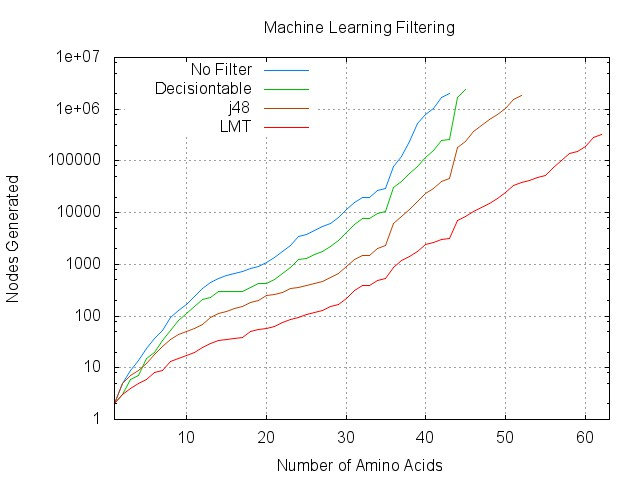
\includegraphics{ProFix_full}}%
    \gplfronttext
  \end{picture}%
\endgroup
}
	\end{center}
\end{figure}

The impact of proline identification on our algorithm's performance is shown in Figure~\ref{fig:figure2}. The same unfiltered and LMT data from Figure~\ref{fig:figure1} is plotted for comparison. The large jump in assignment time between 32 and 33 residue long sequences shows the performance impact of missing data on performance without filtering and using the LMT model for filtering. In the sequence of the studied protein, residue 33 is a proline, for which chemical shifts are missing. If the algorithm identifies and handles prolines as a special case, only one more node is generated for the 33-residue long sequence. However, if the proline is not dealt with separately, the algorithm's performance is significantly impacted. Without proline checking, the proline tile is placed in every position in the assignment. The result is a major increase in the branching factor that leads to the jump observed in Figure~\ref{fig:figure2}. With proline checking, prolines are no longer problematic to the assignment process. This indicates that our algorithm can accurately reproduce assignments with reasonably fast assignment times even when chemical shift data is missing. 

\begin{figure}[H]
	\caption{Impact of proline identification on assignment time. Number of nodes (y-axis) as a function of number of residues used in the assignment (x-axis). Blue shows the search with proline checking and without machine learning filtering. Similarly, the search without either proline checking or machine learning filtering is depicted in purple. The search with proline checking and LMT machine learning filtering is depicted in red. Not utilizing proline checking, but using LMT machine learning filtering is depicted in green.}
	\label{fig:figure2}
	\begin{center}
		\resizebox{!}{0.6\textwidth}{% GNUPLOT: LaTeX picture with Postscript
\begingroup
  \makeatletter
  \providecommand\color[2][]{%
    \GenericError{(gnuplot) \space\space\space\@spaces}{%
      Package color not loaded in conjunction with
      terminal option `colourtext'%
    }{See the gnuplot documentation for explanation.%
    }{Either use 'blacktext' in gnuplot or load the package
      color.sty in LaTeX.}%
    \renewcommand\color[2][]{}%
  }%
  \providecommand\includegraphics[2][]{%
    \GenericError{(gnuplot) \space\space\space\@spaces}{%
      Package graphicx or graphics not loaded%
    }{See the gnuplot documentation for explanation.%
    }{The gnuplot epslatex terminal needs graphicx.sty or graphics.sty.}%
    \renewcommand\includegraphics[2][]{}%
  }%
  \providecommand\rotatebox[2]{#2}%
  \@ifundefined{ifGPcolor}{%
    \newif\ifGPcolor
    \GPcolortrue
  }{}%
  \@ifundefined{ifGPblacktext}{%
    \newif\ifGPblacktext
    \GPblacktexttrue
  }{}%
  % define a \g@addto@macro without @ in the name:
  \let\gplgaddtomacro\g@addto@macro
  % define empty templates for all commands taking text:
  \gdef\gplbacktext{}%
  \gdef\gplfronttext{}%
  \makeatother
  \ifGPblacktext
    % no textcolor at all
    \def\colorrgb#1{}%
    \def\colorgray#1{}%
  \else
    % gray or color?
    \ifGPcolor
      \def\colorrgb#1{\color[rgb]{#1}}%
      \def\colorgray#1{\color[gray]{#1}}%
      \expandafter\def\csname LTw\endcsname{\color{white}}%
      \expandafter\def\csname LTb\endcsname{\color{black}}%
      \expandafter\def\csname LTa\endcsname{\color{black}}%
      \expandafter\def\csname LT0\endcsname{\color[rgb]{1,0,0}}%
      \expandafter\def\csname LT1\endcsname{\color[rgb]{0,1,0}}%
      \expandafter\def\csname LT2\endcsname{\color[rgb]{0,0,1}}%
      \expandafter\def\csname LT3\endcsname{\color[rgb]{1,0,1}}%
      \expandafter\def\csname LT4\endcsname{\color[rgb]{0,1,1}}%
      \expandafter\def\csname LT5\endcsname{\color[rgb]{1,1,0}}%
      \expandafter\def\csname LT6\endcsname{\color[rgb]{0,0,0}}%
      \expandafter\def\csname LT7\endcsname{\color[rgb]{1,0.3,0}}%
      \expandafter\def\csname LT8\endcsname{\color[rgb]{0.5,0.5,0.5}}%
    \else
      % gray
      \def\colorrgb#1{\color{black}}%
      \def\colorgray#1{\color[gray]{#1}}%
      \expandafter\def\csname LTw\endcsname{\color{white}}%
      \expandafter\def\csname LTb\endcsname{\color{black}}%
      \expandafter\def\csname LTa\endcsname{\color{black}}%
      \expandafter\def\csname LT0\endcsname{\color{black}}%
      \expandafter\def\csname LT1\endcsname{\color{black}}%
      \expandafter\def\csname LT2\endcsname{\color{black}}%
      \expandafter\def\csname LT3\endcsname{\color{black}}%
      \expandafter\def\csname LT4\endcsname{\color{black}}%
      \expandafter\def\csname LT5\endcsname{\color{black}}%
      \expandafter\def\csname LT6\endcsname{\color{black}}%
      \expandafter\def\csname LT7\endcsname{\color{black}}%
      \expandafter\def\csname LT8\endcsname{\color{black}}%
    \fi
  \fi
  \setlength{\unitlength}{0.0500bp}%
  \begin{picture}(7200.00,5040.00)%
    \gplgaddtomacro\gplbacktext{%
      \csname LTb\endcsname%
      \put(814,1804){\makebox(0,0)[r]{\strut{}$10^0$}}%
      \csname LTb\endcsname%
      \put(814,2228){\makebox(0,0)[r]{\strut{}$10^1$}}%
      \csname LTb\endcsname%
      \put(814,2653){\makebox(0,0)[r]{\strut{}$10^2$}}%
      \csname LTb\endcsname%
      \put(814,3077){\makebox(0,0)[r]{\strut{}$10^3$}}%
      \csname LTb\endcsname%
      \put(814,3502){\makebox(0,0)[r]{\strut{}$10^4$}}%
      \csname LTb\endcsname%
      \put(814,3926){\makebox(0,0)[r]{\strut{}$10^5$}}%
      \csname LTb\endcsname%
      \put(814,4351){\makebox(0,0)[r]{\strut{}$10^6$}}%
      \csname LTb\endcsname%
      \put(814,4775){\makebox(0,0)[r]{\strut{}$10^7$}}%
      \csname LTb\endcsname%
      \put(1796,1584){\makebox(0,0){\strut{} 10}}%
      \csname LTb\endcsname%
      \put(2741,1584){\makebox(0,0){\strut{} 20}}%
      \csname LTb\endcsname%
      \put(3686,1584){\makebox(0,0){\strut{} 30}}%
      \csname LTb\endcsname%
      \put(4630,1584){\makebox(0,0){\strut{} 40}}%
      \csname LTb\endcsname%
      \put(5575,1584){\makebox(0,0){\strut{} 50}}%
      \csname LTb\endcsname%
      \put(6520,1584){\makebox(0,0){\strut{} 60}}%
      \put(176,3289){\rotatebox{-270}{\makebox(0,0){\strut{}Nodes Generated}}}%
      \put(3874,1254){\makebox(0,0){\strut{}Number of Amino Acids}}%
    }%
    \gplgaddtomacro\gplfronttext{%
      \csname LTb\endcsname%
      \put(4965,833){\makebox(0,0)[r]{\strut{}No Filter}}%
      \csname LTb\endcsname%
      \put(4965,613){\makebox(0,0)[r]{\strut{}Proline Check No Filter}}%
      \csname LTb\endcsname%
      \put(4965,393){\makebox(0,0)[r]{\strut{}LMT}}%
      \csname LTb\endcsname%
      \put(4965,173){\makebox(0,0)[r]{\strut{}Proline Check LMT}}%
    }%
    \gplbacktext
    \put(0,0){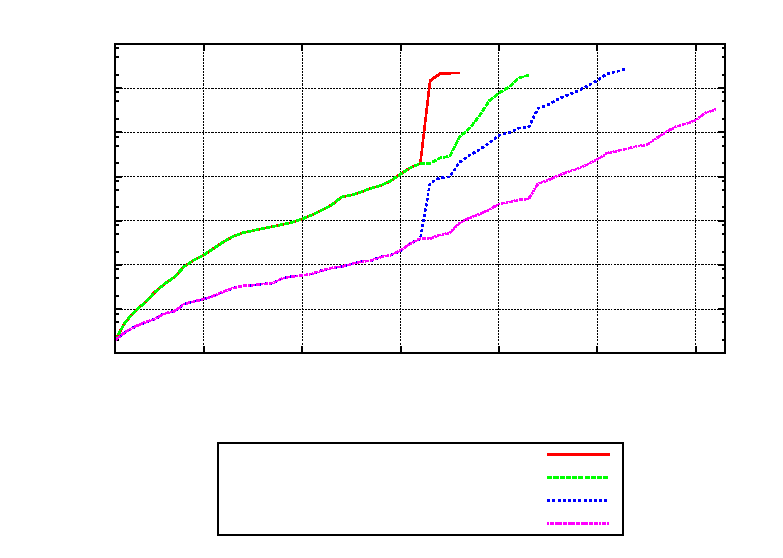
\includegraphics{pro_compare}}%
    \gplfronttext
  \end{picture}%
\endgroup
}
	\end{center}
\end{figure}

Our algorithm with LMT filtering and proline identification can complete the 62-residue assignment in approximately 40 minutes on a 2.3 GHz Intel Core i7 processor with 8Gb of RAM. The LMT model with proline checking can complete the assignment of a 43-residue long sub-sequence in less than 1 second, compared to 27, 29 and 30 seconds without filtering, using a Decision Table for filtering and using the J4.8 model for filtering, respectively. In all cases, the solution from the automated algorithm is identical to the manual assignment, indicating that our algorithm is both fast and accurate. 
\\\\
\noindent\textbf {CONCLUSIONS AND FUTURE DIRECTIONS}\\
Our algorithm has made significant advances in the field of automated assignment of protein backbone chemical shifts. We implemented machine learning to filter NMR data in order to reduce the branching factor in a search-based algorithm. This increased our assignment rate by approximately three orders of magnitude while still maintaining the accuracy of a manually assigned solution.

The use of proline checking and the utilization of machine learning to filter data has shown to be extremely effective in accelerating the assignment. Constrained within the same period of time, reducing the assignment time by 3 orders of magnitude allows for twice as many residues to be assigned. Our algorithm has successfully completed assignments of up to 62 amino acids in a short amount of time and if allotted more time, more residues could be assigned.

One of our main focuses for the future is handling missing data in a more efficient manner. By examining characteristics of the amino acids in the sequence, we hope to predict where missing data will end up in the final assignment. This would reduce the number of assignments attempted. Furthermore, we will look to improve the overall performance of our algorithm by optimizing cost calculations and investigate sequencing via parallel processing.

We are currently measuring the backbone chemical shifts of a protein previously uncharacterized by NMR spectroscopy. This new dataset will include additional chemical shifts that can be used in the assignment process, such as the backbone carbonyl and H-alpha values. This data will be used to further validate and improve our algorithm. Since the cost calculation is crucial to the effectiveness of our algorithm, additional chemical shifts may prove invaluable to the success of the algorithm for longer protein sequences or incomplete datasets. We are also investigating methods of predicting the final cost of an assignment in order to remove unrealistic assignments early on. Having this information available will help optimize our cost calculation, resulting in a further decrease in assignment times. 
\\\\
\textbf{ACKNOWLEDGEMENTS}
\\
The authors of this paper would like to thank Drake University for being a conducive space to research, John Emmons for initiating this research.
\renewcommand{\refname}{\normalfont\selectfont\large \textbf{REFERENCES}}
\bibliographystyle{achemso}
\bibliography{citations}

\vspace{1cm}
\noindent\textbf{ABOUT THE STUDENT AUTHORS}\\
\indent Joel Venzke is a junior pursuing a B.S. in Physics, Computer Science, and  Mathematics. Outside of conducting research, Joel is president of the Drake University chapter of the Society of Physics Students and vice president of the math club. He also works as an award winning photojournalist for Drake University Communications and The Times-Delphic. Joel will be conducting research at Oak Ridge National Lab this summer, and he plans to pursue a PhD in computational science.

David Mascharka is a sophomore seeking a B.S. in Computer Science and Mathematics and B.A. in Philosophy. David also pursues his love for mathematics as the president of the math club at Drake University, where is he able to hone his leadership skills. His research interests include machine learning and mobile computation. David will be spending this summer conducting reasearch at the MIT Haystack Observatory.

Paxten Johnson is on track to graduate in the Spring of 2016 with a B.S. in Physics, Computer Science, and Mathematics. Aside from conducting this research for the past two years, she has been involved with Air Force ROTC, Delta Gamma Fraternity, and the Drake Honor's Program. She hopes to use the knowledge and experience gained from this research to help her advance into the military intelligence branch of the Air Force.

Rachel Davis is currently on the path to obtaining a B.S. in both Computer Science and Mathematics. This is the second year conducting this sequencing research. Her research includes not only this primary structuring of proteins, but also a collaborative tertiary structuring algorithm. Currently she is applying to summer internships closely relating to both her interests and expertise. 

Katie Roth is pursuing a B.A. in Mathematics and Computer Science. She has been working on this research for two years, and enjoys it immensely. Katie is the treasurer of the Women in Mathematics and Computer Science and an active member of Math Club. She is currently applying for summer research experiences, as well as internships. 

Leah Robison is on her way to graduate with a B.S. in Environment Science and a minor in Computer Science. Apart from studying abroad in Denmark for a semester, she has been involved with this research group for the past two years. She hopes to apply the knowledge gained from this research to future studies in the field of Environmental Science.
\\\\
\noindent\textbf{PRESS SUMMARY}\\
Manually assigning nuclear magnetic resonance data to a protein sequence is time consuming and error prone. Although current algorithms have made advances in this area, a student research group at Drake University is improving the process by utilizing machine learning to identify amino acids before assignment. Using both old and new methods has resulted in an algorithm that is fast and accurate. 
\end{document}
